\subsubsection{Generating an object list}
From the detected coordinates $x$ and $y$ and the corresponding distance, the distance, velocity, acceleration, yaw angle of the object and angular velocity, can be calculated. For this previous values are stored and assigned to an \ac{ID}. With the proportionality of the object distance from the vertical center line and the camera angle, the script scales in metric distance.

\begin{equation}
		d_{Pixel} = y_{Pixel} -  \frac{w_{Pixel}}{2}\\	
		\label{eq:d_Pixel}
\end{equation}
\begin{table}[!h]
	\begin{center}
		\begin{tabular}{l c l}
			$d_{Pixel}$ & = & distance from center line to object\\
			$y_{Pixel}$ & = &  y-coordinate of the object\\
			$w_{Pixel}$ & = & pixel format of the video horizontal\\
		\end{tabular}
	\end{center}
\end{table}


\Cref{eq:d_Pixel} divides the image into two segments (left and right segment) and calculates the distance $d_{Pixel}$ of the object to this center axis.

\begin{equation}
k_{angle}  = \frac{d_{Pixel}}{w_{Segment,Pixel}}
\label{eq:k_angle}
\end{equation}
\begin{table}[!h]
	\begin{center}
		\begin{tabular}{l c l}
			$k_{angle}$ & = & proportionality factor for distance and angle\\
			$w_{Segment,Pixel}$ & = &  pixel width of segment\\
		\end{tabular}
	\end{center}
\end{table}

In \cref{eq:k_angle} a factor $k_{angle}$ is calculated which corresponds to a value of -1...0 or 0...1. This factor indicates the object position relative to the total segment width.

\begin{equation}
\phi = k_{angle} * \alpha_{Segment}
\label{eq:phi}
\end{equation}
\begin{table}[!h]
	\begin{center}
		\begin{tabular}{l c l}
			$\phi$ & = & angle from center line to object\\
			$\alpha_{Segment}$ & = &  angle of view for a segment (here: \ang{45})\\
		\end{tabular}
	\end{center}
\end{table}

\begin{figure}[b]
	\centering
	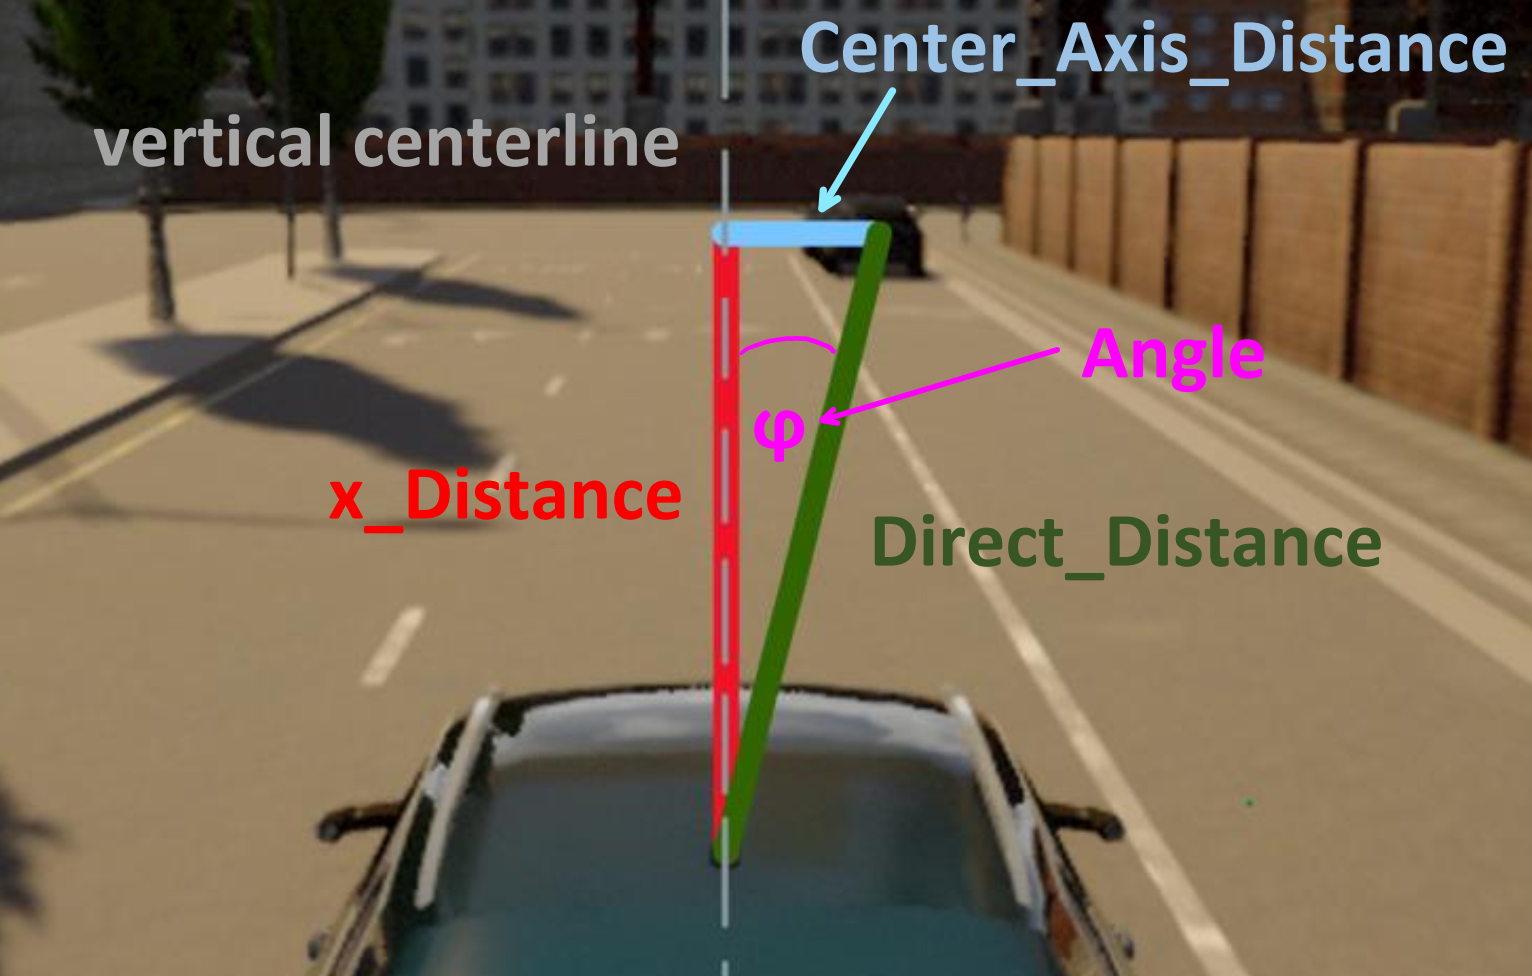
\includegraphics[width=0.4\textwidth]{calc_angle.png}
	\caption{Calculation of angle}
	\label{fig:anglecalculation}
\end{figure}

The field angle of view from the camera which corresponds to \ang{90}, is used. In relation to a segment, it would be \ang{45}. This is calculated with the factor, to get an angle $\phi$ related to the vertical axis (see \cref{eq:phi}).
By using the angle and the direct distance, the trigonometric theorems can be used to calculate the x- and y-distance in meters (shown in \cref{fig:anglecalculation}) which are the basis for the calculation of velocity, acceleration, yaw angle and yaw rate. The object attributes are stored over several frames to calculate time-dependent values. Velocity is calculated by the change of the x- and y-distances, the acceleration, by changing the x- and y-velocities. The yaw angle with the velocity in x- and y-direction and the yaw rate is calculated by time changing angles. The calculated values are related to the ego vehicle.
The dimension of the object is based on formulas \cref{eq:d_Pixel,eq:k_angle,eq:phi} as well. Angle $\phi$ is used to calculate the distance $y$ in meters from the center vertical axis for the position of the vehicle on the y-axis in \cref{eq:y}.

\begin{equation}
	y = h_{direct} * sin(\frac{\phi * \pi}{180})
	\label{eq:y}
\end{equation}
\begin{table}[!h]
	\begin{center}
		\begin{tabular}{l c l}
			$y$ & = & distance from center line to object in meters\\
			$h_{direct}$ & = &  direct distance to object in meters\\
		\end{tabular}
	\end{center}
\end{table}

After calculating the distance of the object to the center axis of the image, it is divided by the pixel distance of the object according to the center axis. This gives a meter per pixel value $k_{MpP}$ to convert the detected object dimensions in pixels to meter (\cref{eq:k_MpP}).

\begin{equation}
	k_{MpP} = \frac{y}{d_{Pixel}}
	\label{eq:k_MpP}
\end{equation}
\begin{table}[!h]
	\begin{center}
		\begin{tabular}{l c l}
			$k_{MpP}$ & = & factor meter per pixel for scaling\\
		\end{tabular}
	\end{center}
\end{table}

With the \ac{ROS} framework, the required data such as geometry, probability, \ac{ID} of the object etc. are transferred via the rose node /data\_play in form of \ac{ROS} message (see \cref{fig:Nodes}).

%\begin{figure}[h]
%	\centering
%	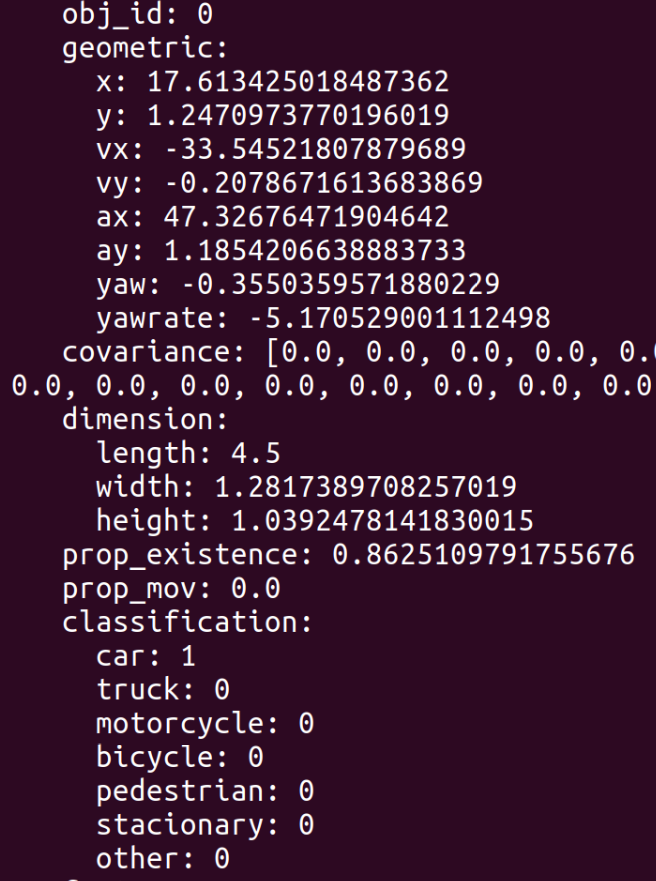
\includegraphics[width=0.3\textwidth]{images/objlist_output.png}
%	\caption{Generated Object List}
%	\label{fig:ros_outout}
%\end{figure}